%!TEX encoding=UTF-8 Unicode
\documentclass[tikz,a4paper,landscape]{standalone}
\usepackage{tikz}
%!TEX encoding=UTF-8 Unicode
%tweeks on pdf version so everybody is happy
\directlua{pdf.setminorversion(4)} % for facile.cines.fr
%\pdfcompresslevel=0 % Not needed


% Libraries
\usetikzlibrary{shapes,arrows,decorations,decorations.pathreplacing,decorations.markings,fit}
\usetikzlibrary{positioning,backgrounds,calc}

\definecolor{StepCol}{HTML}{4575B4}
\definecolor{ObjACol}{HTML}{FC8D59}
\definecolor{ObjAICol}{HTML}{FEE090}
\definecolor{ObjBCol}{HTML}{91BFDB}
\definecolor{ObjBICol}{HTML}{E0F3F8}
\definecolor{ForceCol}{HTML}{D73027}


\tikzset{
  rounded box/.style={
    shape = rectangle,
    draw,
    rounded corners,
    },
  drawed box/.style ={
    rounded box,
    inner sep=.5em,
    draw = #1,
    },
  ObjA-render/.style ={
      circle,
      shading=ball,
      ball color=ObjACol!80!ObjAICol,
      minimum width=1cm,
  },
  ObjA/.style ={
      circle,
      fill=ObjACol,
      minimum width=1cm,
  },
  ObjB/.style ={
      regular polygon,
      regular polygon sides=8,
      fill=ObjBCol,
      minimum width=1cm,
      minimum height=1cm,
  },
  ObjB-render/.style ={
      regular polygon,
      regular polygon sides=8,
      shading=ball,
      ball color=ObjBCol!80!ObjBICol,
      minimum width=1cm,
      minimum height=1cm,
  },
}

\tikzstyle{StepBox} = [drawed box=StepCol]
\tikzstyle{StepA} = [->,StepCol,thick]
\tikzstyle{Force} = [->,ForceCol,thick]

\begin{document}
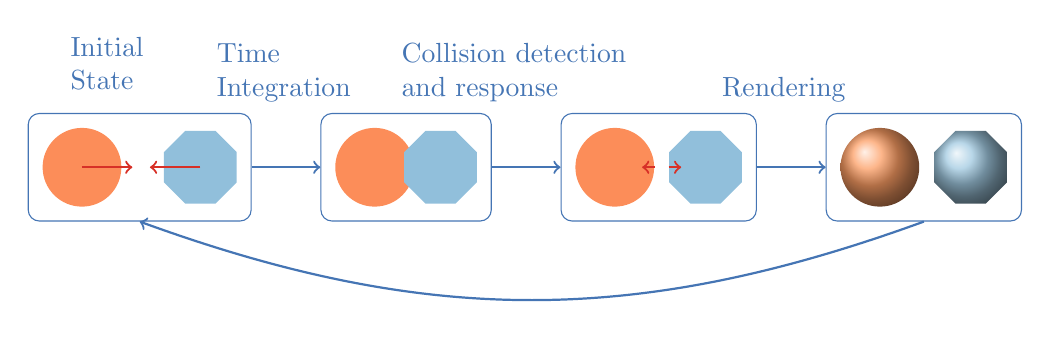
\begin{tikzpicture}[node distance = 2cm,scale=0.8]rotate=90


    \node[ObjA] (Ai) {};
    \node[ObjB,right=15pt of Ai] (Bi) {};

    \node[StepBox,fit=(Ai) (Bi)] (init) {};

    \node[StepCol,text width=5em,above=.5em of init] {Initial\\State};

    \node[ObjA, right=3em of init] (AI) {};
    \node[ObjB,right=-4pt of AI] (BI) {};

    \node[StepBox,fit=(AI) (BI)] (inte) {};


    \node[ObjA, right=3em of inte] (Ac) {};
    \node[ObjB,right=5pt of Ac] (Bc) {};

    \node[StepBox,fit=(Ac) (Bc)] (col) {};

    \node[ObjA-render, right=3em of col] (Ad) {};
    \node[ObjB-render,right=5pt of Ad] (Bd) {};

    \node[StepBox,fit=(Ad) (Bd)] (dis) {};


    % Steps

    \draw[StepA] (init.east) -- node[text width=5em,above=2em]
        {Time\\Integration} (inte.west);

    \draw[StepA] (inte.east) --  node[text width=9em,above=2em]
    {Collision detection\\and response}(col.west) {};

    \draw[StepA] (col.east) -- node[text width=5em,above=2em]
        {Rendering} (dis.west) {};

    %\path[StepA] (col.south) edge[out=-120,in=-60] node[text width=5em,above]
    %    {Collision\\response} (inte.south) {};

    \path[StepA] (dis.south) edge[out=-160,in=-20] (init.south) {};

    % Forces

    \draw[Force] (Ai.center) -- ++(.8,0) {};
    \draw[Force] (Bi.center) -- ++(-.8,0) {};

    \draw[Force] (Ac.east) -- ++(-.2,0) {};
    \draw[Force] (Bc.west) -- ++(.2,0) {};


\end{tikzpicture}
\end{document}
